\item \textbf{{[}HCI/PRELIM/9597/2019/P1/Q4{]} }

A game maintains the player IDs and their scores in an ordered linked
list. The player with the highest score is stored at the first node
while the player with the lowest score is stored at the last node. 

The program to implement the linked list abstract data type will use
two classes, \texttt{ListNode} and \texttt{LinkedList}. 

The \texttt{ListNode} class has the following properties:
\noindent \begin{center}
\begin{tabular}{|l|l|l|}
\hline 
\texttt{\hspace{0.01\columnwidth}}Identifier & \texttt{\hspace{0.01\columnwidth}}Data Type & \texttt{\hspace{0.05\columnwidth}}Description\tabularnewline
\hline 
\texttt{ID} & \texttt{STRING} & The ID of the player. All IDs are unique and have the format \texttt{L999}
where \texttt{L} is any uppercase letter and \texttt{9} is a digit.\tabularnewline
\hline 
\texttt{Score} & \texttt{INTEGER} & The score of the player.\tabularnewline
\hline 
\texttt{Ptr} & \texttt{INTEGER} & The pointer to the next node.\tabularnewline
\hline 
\end{tabular}
\par\end{center}

The \texttt{LinkedList} class has the following properties: 
\noindent \begin{center}
\begin{tabular}{|l|l|l|}
\hline 
\texttt{\hspace{0.01\columnwidth}}Identifier & \texttt{\hspace{0.01\columnwidth}}Data Type & \texttt{\hspace{0.05\columnwidth}}Description\tabularnewline
\hline 
\texttt{Node} & \texttt{ARRAY{[}1..20{]} OF ListNode} & 1-D array stores the nodes that make the ordered linked list. The
unused nodes are linked together into a free list.\tabularnewline
\hline 
\texttt{HeadPtr} & \texttt{INTEGER} & Pointer to the first node in the ordered list.\tabularnewline
\hline 
\texttt{FreePtr} & \texttt{INTEGER} & Pointer to the first node in the free list.\tabularnewline
\hline 
\end{tabular}
\par\end{center}

The following diagram shows an example of a linked list object. This
example list consists of three nodes, linked in descending order of
the game scores. The unused nodes are linked to form a free list.
\begin{center}
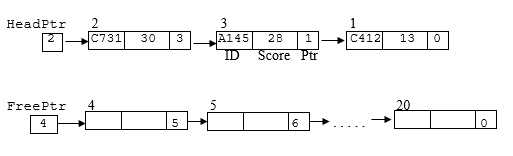
\includegraphics[width=0.5\paperwidth]{C:/Users/Admin/Desktop/Github/question_bank/LyX/static/img/9597-HCI-2019-P1-Q4-1}
\par\end{center}

\subsection*{Task 4.1}

Write program code for the classes \texttt{ListNode} and \texttt{Linkedlist}
to declare all the required variables and create the initial empty
linked list which contains all 20 nodes.

Add statement(s) to initialise the empty ordered linked list.

\subsection*{Evidence 13 }

Your program code for Task 4.1. \hfill{}{[}6{]}

\subsection*{Task 4.2 }

Write code to implement a method \texttt{AddInOrder} that will add
a new node with player\textquoteright s ID and score into the ordered
linked list in descending order of the scores. Node added to the ordered
linked list should be taken from the free list. 

Assume that all players have different scores.

\subsection*{Evidence 14 }

Your program code for Task 4.2.\hfill{} {[}7{]}

\subsection*{Task 4.3 }

Write a procedure \texttt{OutputData} which displays the value of
\texttt{HeadPtr}, the value of \texttt{FreePtr} and the contents of
\texttt{Node} array in index order.

\subsection*{Evidence 15 }

Your program code for Task 4.3.\hfill{} {[}3{]}

The files \texttt{SCORES1.txt} and \texttt{SCORES2.txt} contain the
game data. Each entry has the following format: \texttt{<Player ID>,<Score>} 

\subsection*{Task 4.4 }

Write a main program to:
\begin{itemize}
\item Create a linked list object 
\item Read all player data from \texttt{SCORES1.txt} and add them to the
linked list by calling procedure \texttt{AddInOrder}. 
\item Your program will then call procedure \texttt{OutputData}.
\end{itemize}

\subsection*{Evidence 16 }

Screenshot showing the output from running the program in Task 4.4
using \texttt{SCORES1.txt} file. \hfill{}{[}2{]}

\subsection*{Task 4.5 }

Amend your \texttt{AddInOrder} program code in Task 4.2 so that if
two or more players have the same score, they are stored in alphabetical
player ID order. Use the file \texttt{SCORES2.txt} to test your program
code.

The following diagram shows an example of an ordered linked list where
players \texttt{C412} and \texttt{B321} have the same game score of
\texttt{13} points. 
\begin{center}
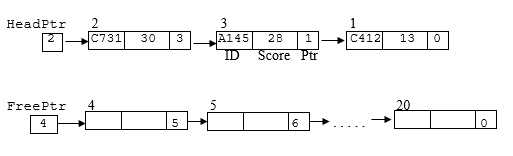
\includegraphics[width=0.5\paperwidth]{C:/Users/Admin/Desktop/Github/question_bank/LyX/static/img/9597-HCI-2019-P1-Q4-1}
\par\end{center}

\subsection*{Evidence 17 }

The amended program code for method \texttt{AddInOrder}. \hfill{}{[}4{]}

\subsection*{Evidence 18}

Screenshot showing the output from running the program in Task 4.4
using \texttt{SCORES2.txt} file. \hfill{}{[}2{]}

\subsection*{Task 4.6 }

A method \texttt{DisplayByRank} is to be added, which outputs all
player IDs and their scores stored in the ordered linked list in rank
order. If multiple players record the same score, they will have the
same rank. 

Below is a sample of screen output:
\noindent \begin{center}
\begin{tabular}{lll}
\texttt{Rank} & \texttt{Player ID} & \texttt{Score}\tabularnewline
\texttt{1} & \texttt{F111} & \texttt{45}\tabularnewline
\texttt{1} & \texttt{G333} & \texttt{45}\tabularnewline
\texttt{1} & \texttt{Z333} & \texttt{45}\tabularnewline
\texttt{4} & \texttt{C333} & \texttt{38}\tabularnewline
\texttt{5} & \texttt{B111} & \texttt{25}\tabularnewline
\texttt{5} & \texttt{Q333} & \texttt{25}\tabularnewline
\texttt{7} & \texttt{E333} & \texttt{12}\tabularnewline
\end{tabular}
\par\end{center}

Write program code to:
\begin{itemize}
\item Implement this method 
\item Test the program code with the data from Task 4.5.
\end{itemize}

\subsection*{Evidence 19 }

Program code for Task 4.6. \hfill{}{[}7{]}

\subsection*{Evidence 20}

Screenshot of the program output.\hfill{} {[}2{]}

\subsection*{Task 4.7 }

Write a recursive \texttt{ReverseTraversal} procedure that will traverse
the linked list in reverse order and output players\textquoteright{}
IDs and scores in ascending scores order.

Include a call to the procedure from your main program.

Test the program code with the data from Task 4.5.

\subsection*{Evidence 21 }

Your program code for Task 4.7.\hfill{}{[}4{]}

\subsection*{Evidence 22}

Screenshot showing the program execution to test the \texttt{ReverseTraversal}
method. \hfill{}{[}2{]}